\section{Brain Organoids and Wetware Computing}

The integration of brain organoids with wetware computing systems presents a powerful paradigm for investigating ECC's principles in controllable yet biologically authentic environments. Brain organoids provide a unique experimental platform through their development of sophisticated cellular architectures that mirror aspects of cortical organization \cite{Lancaster2013}. These three-dimensional neural tissues enable investigation of how coherent energy patterns emerge and evolve within developing networks.

Recent advances in organoid development have demonstrated remarkable capacity for modeling human brain development and organization \cite{Quadrato2017}. These systems can be engineered with specific transcriptomic profiles and cellular compositions optimized for studying coherence dynamics. The incorporation of reporter systems for real-time energy state monitoring enables continuous tracking of how coherent patterns emerge and stabilize within developing neural networks.

The rise of three-dimensional human brain cultures offers unprecedented opportunities for studying consciousness-supporting mechanisms \cite{Pasca2018}. By combining organoid systems with wetware computing elements, researchers can create hybrid platforms that enable precise control over network architecture while maintaining biological authenticity. These approaches provide crucial windows into how consciousness-supporting mechanisms emerge from biological organization.

The marriage of biological and computational elements in wetware systems draws on fundamental principles of molecular coordination in living systems \cite{MacLennan2009}. These hybrid approaches demonstrate how information processing can emerge directly from physical dynamics rather than requiring implementation through traditional computational architectures. The success of biological computation in systems like Physarum demonstrates sophisticated information processing capabilities emerging from natural physical dynamics \cite{Adamatzky2016}.

The efficiency scaling in biological versus programmable systems reveals important principles about consciousness-supporting architectures \cite{Conrad1995}. Unlike traditional computational approaches that rely on discrete state transitions, biological systems achieve sophisticated information processing through continuous physical dynamics. This distinction proves crucial for understanding how conscious processing emerges from coherent energy states.

The bioelectric code provides another essential framework for understanding how biological systems achieve sophisticated information processing \cite{Levin2018}. Through careful regulation of bioelectric signaling, cellular networks can maintain coherent states that enable complex computation. These insights prove particularly valuable for developing hybrid systems capable of supporting consciousness-like processing.

\begin{figure}[h]
    \centering
    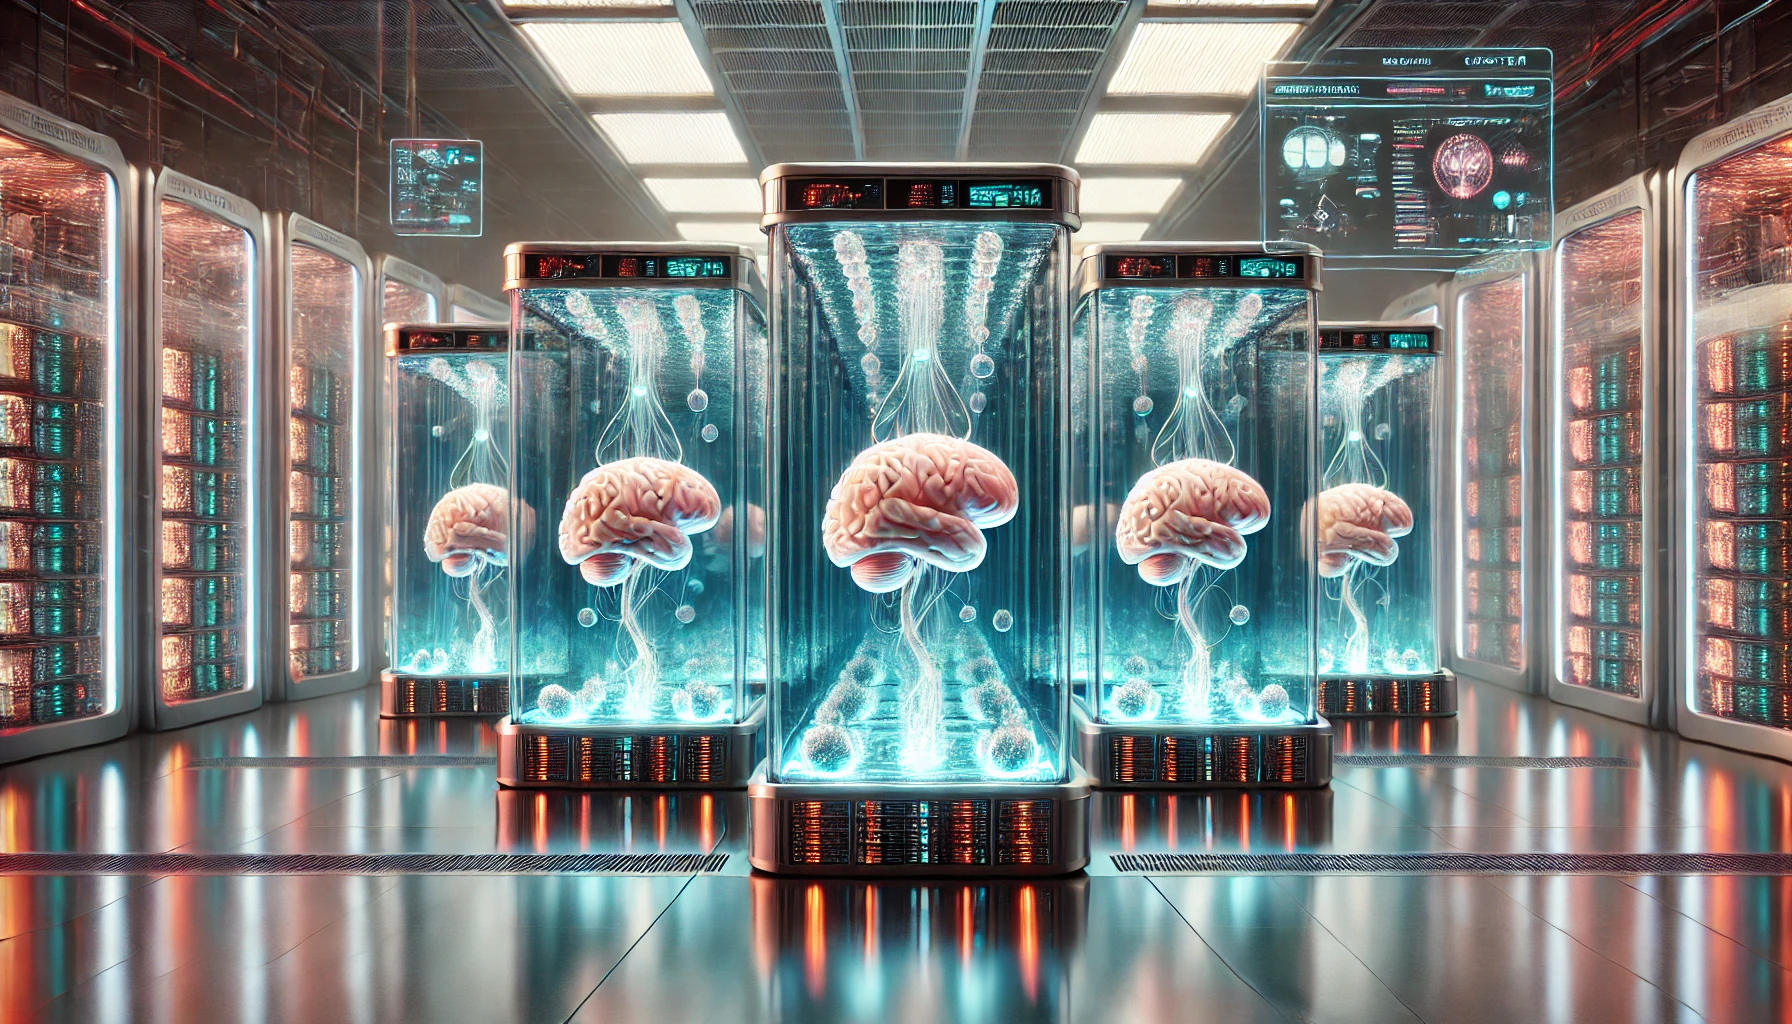
\includegraphics[width=0.8\textwidth]{organoids.png}

    \caption{A dystopic portrayal of a brain organoid data center.}
\end{figure}

The integration of biological and computational principles requires careful attention to how physical systems achieve information processing. Studies of bioelectric signaling reveal sophisticated mechanisms for controlling growth and form in biological tissues \cite{Levin2018}. These bioelectric codes demonstrate how living systems implement computation through direct physical processes rather than abstract symbol manipulation.

Advanced simulation tools enable systematic investigation of physiological signaling in biological tissues \cite{Pietak2017}. These platforms help researchers understand how coherent patterns emerge from complex cellular interactions, providing crucial insights into consciousness-supporting mechanisms. The ability to model and manipulate bioelectric fields offers new approaches for studying how conscious-like processing might emerge in engineered biological systems.

Recent developments in neuromorphic computing have demonstrated remarkable capabilities in artificial neural systems \cite{Merolla2014}. However, these digital implementations fundamentally differ from biological computation in their physical implementation. Understanding these differences helps clarify why consciousness may require specific forms of biological organization rather than merely sophisticated information processing.

The integration of living neural networks with artificial systems presents unique opportunities for investigating consciousness-supporting mechanisms \cite{DeMarse2005}. These hybrid approaches enable systematic examination of how biological neural networks achieve and maintain coherent states while processing information. The ability to interface living neurons with artificial systems provides valuable tools for testing ECC's predictions about consciousness-supporting architectures.

Ethical considerations become increasingly relevant as brain organoids achieve greater sophistication. Recent work has raised important questions about consciousness assessment in cerebral organoids \cite{Lavazza2018}. These ethical challenges require careful consideration as researchers develop more complex biological systems capable of supporting consciousness-like processing.

The experimental use of human brain tissue demands rigorous ethical frameworks \cite{Farahany2018}. As organoid systems become more sophisticated, researchers must carefully consider the potential for conscious-like properties to emerge in these tissues. This ethical dimension becomes particularly significant when developing systems specifically designed to test theories of consciousness.

\begin{figure}[h]
    \centering
    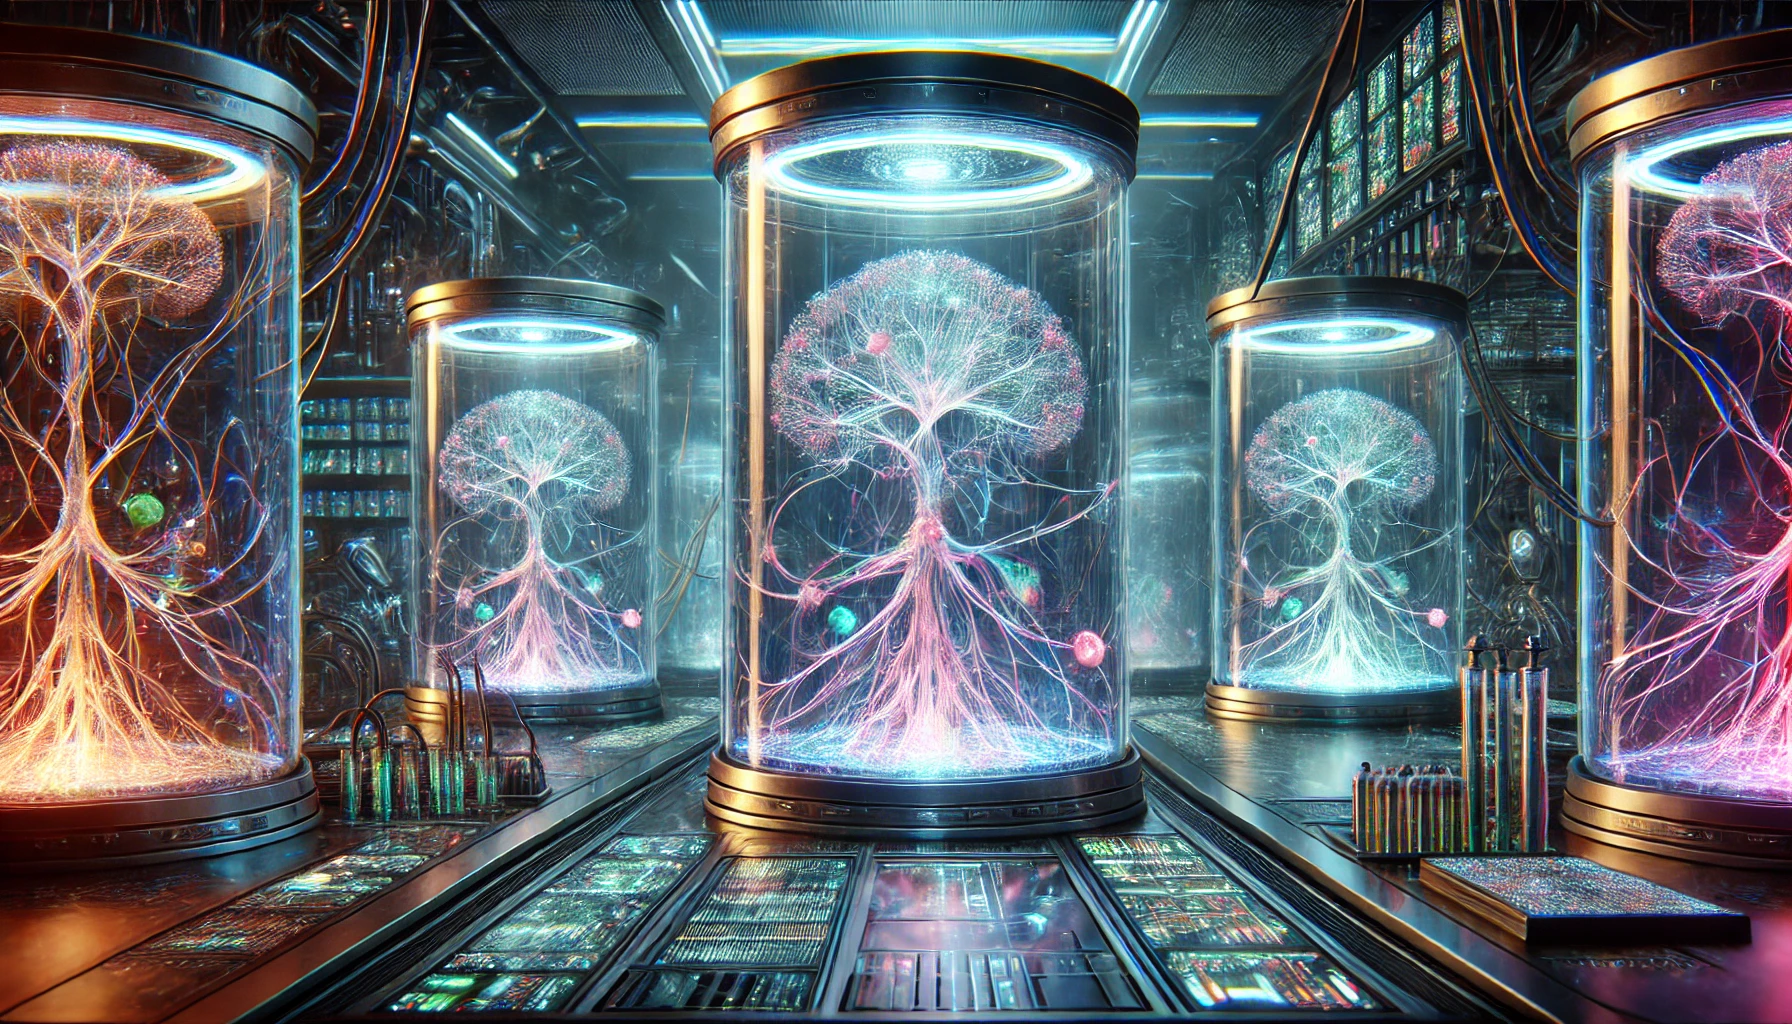
\includegraphics[width=0.8\textwidth]{wetware.png}

    \caption{Wetware computing}
\end{figure}

The integrated systems approach to biological networks reveals fundamental principles about how consciousness-supporting architectures emerge from neural organization \cite{Zhang2016}. By examining how different cellular elements interact to create coherent states, researchers can better understand the physical requirements for conscious processing. This systems-level perspective proves essential for bridging between molecular mechanisms and conscious experience.

Recent work has illuminated how conscious integration depends on physical substrates rather than abstract computation \cite{Krishnan2019}. The specific properties of biological tissues enable forms of information processing that cannot be reduced to traditional computational approaches. Understanding these physical constraints helps explain why consciousness requires particular forms of biological organization.

Advanced organoid and assembloid technologies provide increasingly sophisticated platforms for investigating neural development and function \cite{Saha2020}. These systems enable systematic examination of how neural tissues achieve and maintain coherent states through biological mechanisms. The ability to create more complex neural structures offers new opportunities for studying consciousness-supporting architectures.

The development of bioengineered functional brain-like cortical tissue represents a significant advancement for consciousness research \cite{TangSchomer2014}. These engineered tissues demonstrate how biological systems can achieve sophisticated information processing through direct physical mechanisms rather than abstract computation. Such approaches align with ECC's emphasis on consciousness as emerging from coherent energy dynamics in biological systems.

The future development of brain organoids and wetware computing must carefully balance scientific advancement with ethical considerations. As these systems become more sophisticated, researchers must remain attentive to both the potential for conscious-like properties to emerge and the implications of creating such systems. This careful integration of scientific and ethical considerations will prove essential for advancing our understanding of consciousness while maintaining responsible research practices.